\subsection{Docking}
    \begin{task}[label=task:Docking]{Docking a ligand into the protein.}
        \begin{enumerate}[label=(\alph*)]
            \item Dock the ligand
            \item Check docked poses
        \end{enumerate}
    \end{task}

    \paragraph{}
        To run a \gls{acr:md} simulation of a ligand-protein complex, you first need a good start structure for the ligand docked into the protein. Luckily many protein structures are obtained with a ligand already docked into the active site and so these positions can be used as a starting point for docking our ligands. We shall be using gnina as it can take the \enquote{2BN.pdb} structure generated previously as an initial guess for the active site location.

    \begin{bashcmd}[label=cmd:gnina]{Basic input for gnina without GPU acceloration}
        gnina -r 1n23_monomer_NoLig.pdb -l LIG.mol2 --autobox_ligand 2BN.pdb  -o docked.mol2 --no_gpu 
    \end{bashcmd}

    \begin{table}[H]
    \centering
    \begin{tabular}{@{}cll@{}}
    \toprule
    \multicolumn{1}{l}{\textbf{Option}} & \textbf{Value}    & \textbf{Type} \\ \midrule
    \textendash r                                           & Receptor/Protein pdb file                 & Input     \\
    \textendash l                                           & Ligand file to be docked                  & Input     \\
    \textendash \textendash autobox\textunderscore ligand   & Stripped receptor/protein parameter file  & Input     \\
    \textendash o                                           & Output PDB file for docked poses          & Output    \\
    \textendash \textendash no\textunderscore gpu           & Switches off GPU acceleration             & Variable  \\
                                                            & (Not necessary if compiled correctly)    &           \\
    \bottomrule
    \end{tabular}
    \label{Tab:gninaVar}
    \caption{The input variables for gnina}
    \end{table}

    \paragraph{}
    The docked poses of the ligand can then be viewed using \texttt{VMD}, like when viewing the original complexed structure. You will however need to load in two files rather than one. It is easiest if you load your \enquote{1n23\textunderscore monomer\textunderscore NoLig.pdb} file first, then open the \enquote{docked.mol2} file once \texttt{VMD} has loaded (Figures \ref{fig:NewMol} and \ref{fig:LoadMol}). This will set the docked structures as \enquote{on top} meaning you can cycle through the different docked \enquote{Frames}. You should set your representation for your protein as \enquote{New Cartoon} (Figure \ref{fig:protRep}) and the representation for your docked ligand as \enquote{CPK} (Figure \ref{fig:dockRep}). 
        
    \begin{figure}[H]
        \centering
        \begin{minipage}{0.45\textwidth}
            \centering
            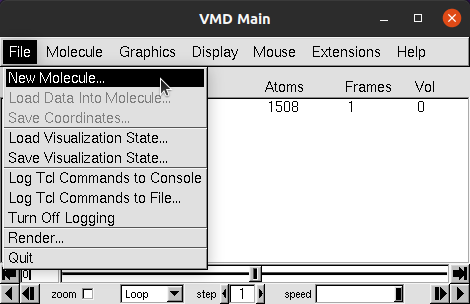
\includegraphics[width=0.9\textwidth]{Graphics/ScreenShots/NewMol.png}
            \captionof{figure}{How to load a new \\ molecule in VMD.}
            \label{fig:NewMol}
        \end{minipage}%
        \begin{minipage}{0.45\textwidth}
            \centering
            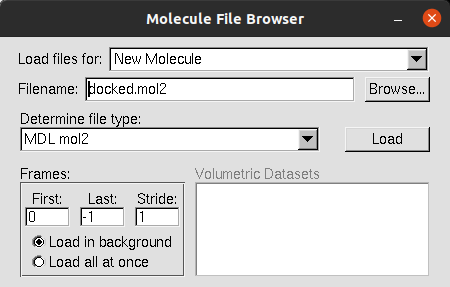
\includegraphics[width=0.9\textwidth]{Graphics/ScreenShots/docked_file.png}
            \captionof{figure}{How to select the file.}
            \label{fig:LoadMol}
        \end{minipage}
    \end{figure}

    \begin{figure}[H]
        \centering
        \begin{minipage}{0.45\textwidth}
            \centering
            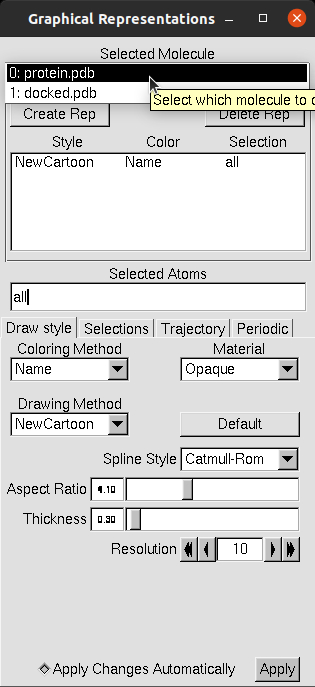
\includegraphics[height=0.5\textheight]{Graphics/ScreenShots/protein.png}
            \captionof{figure}{The representation for the protein.}
            \label{fig:protRep}
        \end{minipage}%
        \begin{minipage}{0.45\textwidth}
            \centering
            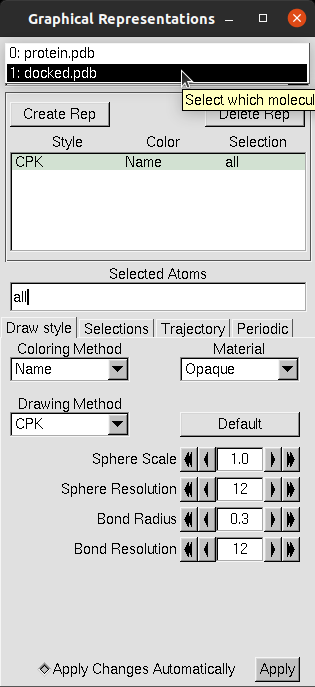
\includegraphics[height=0.5\textheight]{Graphics/ScreenShots/docked.png}
            \captionof{figure}{The representation for the \\ docked ligand.}
            \label{fig:dockRep}
        \end{minipage}
    \end{figure}

    \paragraph{}
        Finally, to use the docked pose for the molecular dynamics simulation you must extract the initial pose from the output coordinate file. You can either do this through the \gls{acr:gui} in VMD, or through the \gls{acr:cli}. It is recommended to use the \gls{acr:cli} as this is the fastest method and ensures that no structural manipulation takes place. To do this you copy the \enquote{docked.mol2} file to \enquote{pose\textunderscore 1.mol2}, then open in either vim or nano. From there you can simply delete the other docked poses from the file. (All the lines from the second \enquote{@<TRIPOS>MOLECULE}). The final docked file should look something similar to File \ref{out:mol2}.

    \begin{bashoutput}[label=out:mol2]{Docked pose output file.}
@<TRIPOS>MOLECULE
LIG.xyz
 10 9 0 0 0
SMALL
GASTEIGER

@<TRIPOS>ATOM
      1 C  42.7160   46.4533   46.0135 C.3     1  UNL1        0.0090
      2 C  43.7928   47.2054   46.6251 C.3     1  UNL1        0.0224
      3 C  43.7468   48.6707   46.5384 C.3     1  UNL1        0.0047
      4 C  44.7948   45.1707   47.5267 C.2     1  UNL1       -0.0049
      5 C  44.8573   46.4823   47.2270 C.2     1  UNL1       -0.0265
      6 C  41.4018   46.7840   46.8568 C.3     1  UNL1        0.0257
      7 C  41.7288   46.7347   48.3034 C.2     1  UNL1       -0.0346
      8 C  41.7967   45.6383   49.0677 C.2     1  UNL1       -0.0478
      9 C  42.1951   45.7469   50.5025 C.3     1  UNL1        0.0260
     10 C  41.5150   44.2497   48.5990 C.3     1  UNL1        0.0260
@<TRIPOS>BOND
     1     4     5    2
     2     5     2    1
     3     2     3    1
     4     2     1    1
     5     1     6    1
     6     6     7    1
     7     7     8    2
     8     8     9    1
     9     8    10    1
    \end{bashoutput}

    \paragraph{}
        You will notice that this docking procedure has removed the protons from our ligand so we shall have to manually add them back in. As our ligand is a carbocation, this process is more complicated than normal as automating the protonation of the molecule will also neutralise it. One way to fix this is to protonate the ligand to the neutral molecule, then manually remove the proton using a text editor. As \enquote{mol2} files contain bonding information, it is best to do this with a \enquote{.xyz} molecule file however.

    \begin{bashcmd}[label=cmd:addH]{Add hydrogen atoms and convert to .xyz.}
        obabel -imol2 pose_1.mol2 -oxyz -Opose_1.xyz -h   
        #This protonates and converts to xyz in one step.
    \end{bashcmd}

    \begin{bashoutput}[label=out:xyz]{Protonated neutral ligand.}
28
LIG.xyz
C         42.71600       46.45330       46.01350
C         43.79280       47.20540       46.62510
C         43.74680       48.67070       46.53840
C         44.79480       45.17070       47.52670
C         44.85730       46.48230       47.22700
C         41.40180       46.78400       46.85680
C         41.72880       46.73470       48.30340
C         41.79670       45.63830       49.06770
C         42.19510       45.74690       50.50250
C         41.51500       44.24970       48.59900
H         42.92737       45.40513       46.05305
H         42.59360       46.71744       44.98387
H         44.18007       47.67066       47.50740
H         43.32922       48.95932       45.59647
H         44.73798       49.06439       46.62478
H         43.13968       49.05599       47.33077
H         45.60368       44.70221       47.96403
H         43.93803       44.63420       47.31901
H         45.72789       46.99089       47.44709
H         40.64322       46.06240       46.63601
H         41.04477       47.75962       46.60067
H         41.92334       47.63624       48.76643
H         42.37555       46.77311       50.74586
H         43.08636       45.17877       50.66917
H         41.40891       45.36665       51.12073
H         41.23917       44.27121       47.56539
H         40.71320       43.83510       49.17356
H         42.39066       43.64721       48.72201
    
    \end{bashoutput}

    \paragraph{}
        When visualising the file, you will see that there is a proton on the carbocation. Selecting this atom shows us that it is atom index 12 and as \texttt{vmd} is \enquote{zero indexed}, it is the 13\textsuperscript{th} atom which needs removing. Delete this line in the \enquote{pose\textunderscore 1.xyz} file, and change the number at the top from 28 to 27 as this is the number of atoms in the molecule. Finally, we will convert back to \enquote{mol2} using obabel and \cref{cmd:xyzmol2}.

    \begin{bashcmd}[label=cmd:xyzmol2]{Convert back to mol2.}
        obabel -ixyz pose_1.xyz -omol2 -Opose_1.mol2
    \end{bashcmd}


    \paragraph{}
        Finally, you need to check that the hybridisation states for all of the carbons are correct. There should be 5 \enquote{C.2} carbons as there are 2 double bonds and 1 cationic carbon atom. It is likely that obabel incorrectly identified the carbocation as \enquote{C.2} and so you should manually change this in your file (the carbocation should be carbon 2). The final file should look something like \cref{out:finaldocked} however we have excluded the bonding information for simplicity.

    \begin{bashoutput}[label=out:finaldocked]{The final structure for the docked molecule.}
@<TRIPOS>MOLECULE
LIG.xyz
 27 26 0 0 0
SMALL
GASTEIGER

@<TRIPOS>ATOM
    1 C  42.7160   46.4533   46.0135 C.3    1  UNL1    -0.0400
    2 C  43.7928   47.2054   46.6251 C.2    1  UNL1    -0.0052
    3 C  43.7468   48.6707   46.5384 C.3    1  UNL1    -0.0553
    4 C  44.7948   45.1707   47.5267 C.2    1  UNL1    -0.1021
    5 C  44.8573   46.4823   47.2270 C.2    1  UNL1    -0.0844
    6 C  41.4018   46.7840   46.8568 C.3    1  UNL1    -0.0337
    7 C  41.7288   46.7347   48.3034 C.2    1  UNL1    -0.0853
    8 C  41.7967   45.6383   49.0677 C.2    1  UNL1    -0.0796
    9 C  42.1951   45.7469   50.5025 C.3    1  UNL1    -0.0440
   10 C  41.5150   44.2497   48.5990 C.3    1  UNL1    -0.0440
   11 H  42.9274   45.4051   46.0530 H      1  UNL1     0.0277
   12 H  42.5936   46.7174   44.9839 H      1  UNL1     0.0277
   13 H  43.3292   48.9593   45.5965 H      1  UNL1     0.0238
   14 H  44.7380   49.0644   46.6248 H      1  UNL1     0.0238
   15 H  43.1397   49.0560   47.3308 H      1  UNL1     0.0238
   16 H  45.6037   44.7022   47.9640 H      1  UNL1     0.0532
   17 H  43.9380   44.6342   47.3190 H      1  UNL1     0.0532
   18 H  45.7279   46.9909   47.4471 H      1  UNL1     0.0572
   19 H  40.6432   46.0624   46.6360 H      1  UNL1     0.0308
   20 H  41.0448   47.7596   46.6007 H      1  UNL1     0.0308
   21 H  41.9233   47.6362   48.7664 H      1  UNL1     0.0571
   22 H  42.3755   46.7731   50.7459 H      1  UNL1     0.0274
   23 H  43.0864   45.1788   50.6692 H      1  UNL1     0.0274
   24 H  41.4089   45.3666   51.1207 H      1  UNL1     0.0274
   25 H  41.2392   44.2712   47.5654 H      1  UNL1     0.0274
   26 H  40.7132   43.8351   49.1736 H      1  UNL1     0.0274
   27 H  42.3907   43.6472   48.7220 H      1  UNL1     0.0274
@<TRIPOS>BOND
 # Bonding information
    \end{bashoutput}